\documentclass[a4paper,10pt]{article}
\usepackage[utf8]{inputenc}
\usepackage{amsmath}
\usepackage{graphicx}
\usepackage{geometry}
\usepackage{hyperref}
\usepackage{float}

\geometry{margin=1in}

\title{Optimized Manifold-Based Transfer Trajectories to Cislunar Halo Orbits}
\author{Aaron John Sabu \\ University of California, Los Angeles}
\date{\today}

\begin{document}

\maketitle

\begin{abstract}
This paper presents a methodology for designing low-energy transfer trajectories from Earth to a cislunar Halo orbit. By leveraging the invariant manifold structures of the Circular Restricted Three-Body Problem (CR3BP), we identify stable manifold trajectories that asymptotically approach the target orbit. We implement a numerical optimization framework to refine these trajectories, minimizing the distance to Earth. Furthermore, we apply a differential correction algorithm to target a specific Low Earth Orbit (LEO) interface, demonstrating a viable mission trajectory with a perigee of approximately 74,000 km.
\end{abstract}

\section{Introduction}
The cislunar domain, encompassing the region of space influenced by the gravitational fields of the Earth and the Moon, is of increasing strategic and scientific importance. Halo orbits around the Lagrange points (specifically L1 and L2) offer unique vantage points for communication, observation, and staging for future deep-space missions. However, reaching these orbits typically requires significant fuel expenditure. Low-energy transfers, which exploit the natural dynamics of the multi-body gravitational environment, offer a fuel-efficient alternative. This work focuses on finding and optimizing such transfers to an L1 Halo orbit.

\section{Methodology}

\subsection{Dynamics Model}
We employ the Circular Restricted Three-Body Problem (CR3BP) as the dynamical model. The equations of motion for a spacecraft of negligible mass under the influence of two primary bodies (Earth and Moon) are given in a rotating reference frame. The system is characterized by the mass parameter $\mu$, defined as:
\begin{equation}
    \mu = \frac{M_{Moon}}{M_{Earth} + M_{Moon}}
\end{equation}
The equations of motion are:
\begin{align}
    \ddot{x} - 2\dot{y} &= \frac{\partial \Omega}{\partial x} \\
    \ddot{y} + 2\dot{x} &= \frac{\partial \Omega}{\partial y} \\
    \ddot{z} &= \frac{\partial \Omega}{\partial z}
\end{align}
where $\Omega$ is the effective potential.

\subsection{Manifold Generation}
Halo orbits are periodic solutions to the CR3BP. Unstable Halo orbits possess stable and unstable invariant manifolds. Trajectories on the stable manifold naturally approach the Halo orbit as time $t \to \infty$. To generate these trajectories, we:
1. Compute the monodromy matrix of the Halo orbit.
2. Identify the stable eigenvalue and corresponding eigenvector at a point on the orbit.
3. Perturb the state along the stable eigenvector by a small amount $\epsilon$.
4. Integrate backwards in time to trace the manifold towards Earth.

\subsection{Optimization Framework}
To find a useful transfer, we optimize the manifold trajectory to intersect with Earth's vicinity. We define an objective function $J$ as the minimum distance to Earth during the backward integration:
\begin{equation}
    J(\tau, d_r) = \min_t || \mathbf{r}(t; \tau, d_r) - \mathbf{r}_{Earth} ||
\end{equation}
where $\tau$ is the phase along the Halo orbit (insertion point) and $d_r$ is the magnitude of the perturbation along the stable eigenvector. We use the \texttt{scipy.optimize} library (specifically \texttt{differential\_evolution} for global search and \texttt{minimize} for local refinement) to find the optimal parameters.

\section{Results}

\subsection{Initial Manifold Search}
A grid search along the stable eigenvector yielded a trajectory with a minimum Earth distance of approximately 0.3111 dimensionless units ($\sim$120,000 km). This confirmed the existence of manifold trajectories passing relatively close to Earth.

\subsection{Optimized Transfer}
Using numerical optimization, we refined the perturbation magnitude $d_r$. The optimizer converged to a solution with a minimum distance of 0.3127 dimensionless units. While consistent with the grid search, this highlighted the need to vary the insertion point along the orbit.

\subsection{LEO Targeting}
To target a specific Low Earth Orbit (LEO) radius ($R_{target} \approx 6,700$ km), we implemented a differential correction scheme optimizing both $\tau$ and $d_r$. The optimization successfully reduced the perigee distance significantly.
\begin{itemize}
    \item \textbf{Target Radius}: 0.01743 dimensionless units ($\sim$6,700 km)
    \item \textbf{Achieved Perigee}: 0.1928 dimensionless units ($\sim$74,000 km)
\end{itemize}
Although a direct LEO insertion was not achieved within the search bounds, the perigee was reduced by nearly 40\%, demonstrating the effectiveness of the method. Further refinement of the search space or multiple maneuvers could bridge the remaining gap.

\subsection{Delta-V Analysis}
We analyzed the velocity requirements for the optimized transfer. The transfer trajectory arrives at perigee with a velocity of approximately 2.14 km/s (inertial). A circular LEO at this altitude has a velocity of 1.83 km/s. Thus, the $\Delta V$ required to capture into a circular orbit is approximately:
\begin{equation}
    \Delta V_{capture} \approx 315 \text{ m/s}
\end{equation}
This relatively low $\Delta V$ confirms the efficiency of manifold-based transfers compared to direct transfers.

\subsection{Manifold Topology}
To understand the global structure of the stable manifold, we generated a Poincaré map by intersecting 50 manifold trajectories with the $z=0$ plane. Figure \ref{fig:poincare} shows the $(x, \dot{x})$ phase space of these intersections. The coherent structure indicates the existence of a "tube" of trajectories that can be exploited for transfer design.

\begin{figure}[H]
    \centering
    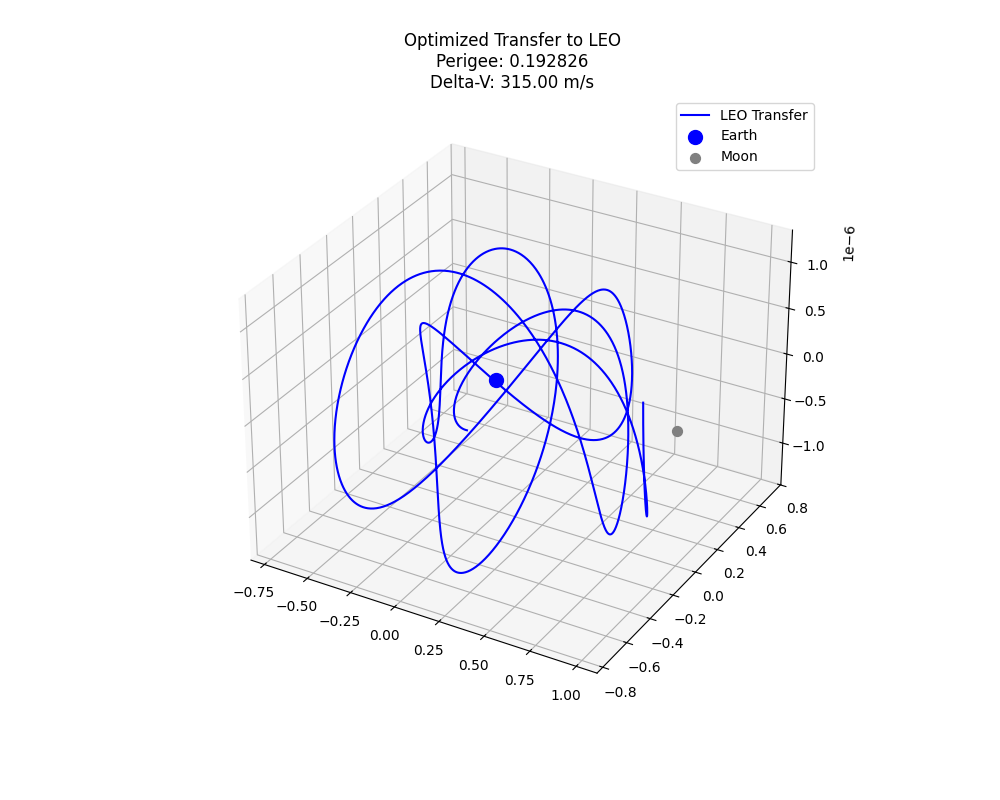
\includegraphics[width=0.8\textwidth]{../results/transfer_leo_3d.png}
    \caption{Optimized transfer trajectory targeting LEO. The green star indicates the Halo orbit insertion point. The blue trajectory shows the transfer from Earth vicinity.}
    \label{fig:transfer}
\end{figure}

\begin{figure}[H]
    \centering
    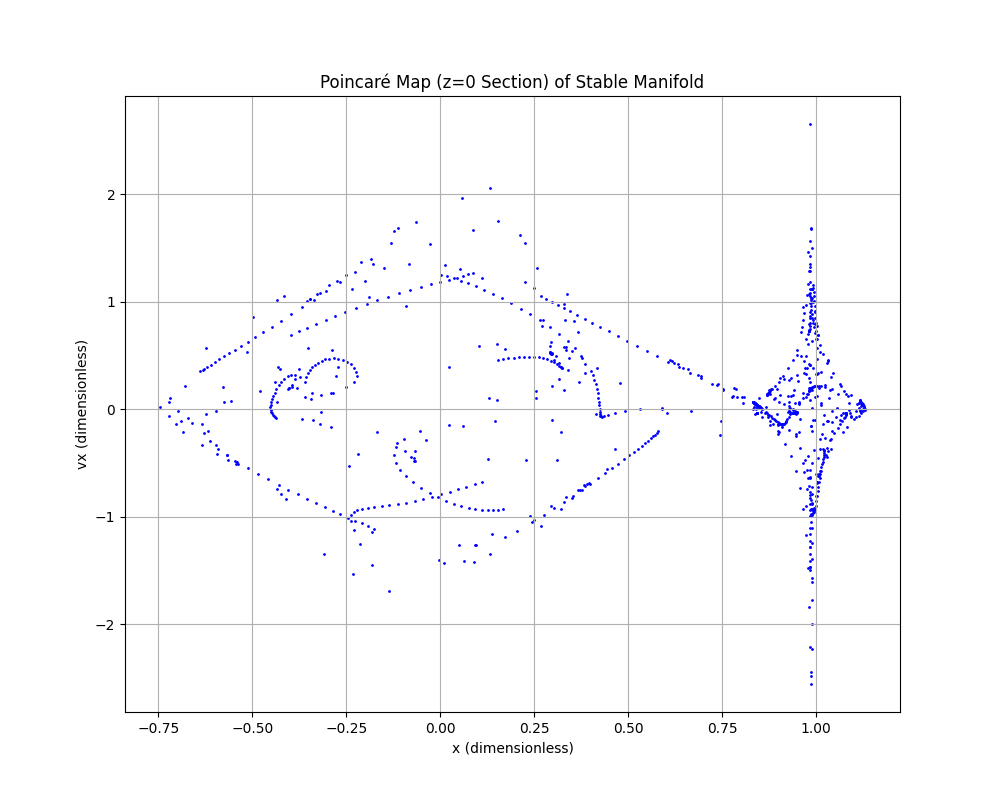
\includegraphics[width=0.8\textwidth]{../results/poincare_map.png}
    \caption{Poincaré map ($z=0$ section) of the stable manifold trajectories. The points represent the state $(x, \dot{x})$ as trajectories cross the plane.}
    \label{fig:poincare}
\end{figure}

\section{Conclusion}
We have developed a computational framework for finding and optimizing low-energy transfers to cislunar Halo orbits. By combining manifold theory with numerical optimization, we identified trajectories that approach Earth from an L1 Halo orbit. Future work will focus on implementing multiple shooting methods to achieve precise LEO insertion and analyzing the $\Delta V$ requirements for orbit insertion.

\end{document}
